\subsection{Approssimazione di derivate}

Al fine di approssimare il problema di Cauchy, è necessario prima introdurre un altro problema: \textbf{siano noti i valori $v\left(t_{n}\right)$ di una funzione $v$ in corrispondenza di noti $t_{n}$, $n=0, \dots, N$, e si vuole approssimare i valori della sua derivata prima $v'\left(t\right)$ negli stessi nodi}.

\highspace
\begin{flushleft}
	\textcolor{Red2}{\faIcon{bookmark} \textbf{Approssimazione in avanti della derivata prima}}
\end{flushleft}
Partendo dallo sviluppo in serie di Taylor:
\begin{equation*}
	v\left(t_{n+1}\right) = v\left(t_{n}\right) + hv'\left(t_{n}\right) + \dfrac{h^{2}}{2} v''\left(t_{n}\right) + \dfrac{h^{3}}{6} v'''\left(t_{n}\right) + O\left(h^{4}\right)
\end{equation*}
E ricordando che una quantità è un $O\left(h^{p}\right)$ se vale:
\begin{equation*}
	\lim\limits_{h \rightarrow 0} \dfrac{O\left(h^{p}\right)}{h^{p}} < +\infty
\end{equation*}
Ovverosia se va a $0$ con la stessa velocità o più velocemente di $h^{p}$. Scrivendo la derivata $v'\left(t_{n}\right)$ come:
\begin{equation*}
	v'\left(t_{n}\right) = \dfrac{v\left(t_{n+1}\right) - v\left(t_{n}\right)}{h} - \underbrace{
		\dfrac{h}{2} v''\left(t_{n}\right) - \dfrac{h^{2}}{6} v'''\left(t_{n}\right) + O\left(h^{3}\right)
	}_{O\left(h\right)}
\end{equation*}
Questo consente di introdurre un'\definition{approssimazione in avanti della derivata prima}:
\begin{equation}\label{eq: approssimazione in avanti della derivata prima}
	D^{+}v\left(t_{n}\right) = \dfrac{v\left(t_{n+1}\right) - v\left(t_{n}\right)}{h}
\end{equation}
Il cui \textbf{errore} è dato da:
\begin{equation}
	\left|v'\left(t_{n}\right) - D^{+}v\left(t_{n}\right)\right| = O\left(h\right)
\end{equation}

\highspace
\begin{flushleft}
	\textcolor{Red2}{\faIcon{bookmark} \textbf{Approssimazione all'indietro della derivata prima}}
\end{flushleft}
In modo analogo, considerando il seguente sviluppo di Taylor:
\begin{equation*}
	v\left(t_{n-1}\right) = v\left(t_{n}\right) + hv'\left(t_{n}\right) + \dfrac{h^{2}}{2} v''\left(t_{n}\right) + \dfrac{h^{3}}{6} v'''\left(t_{n}\right) + O\left(h^{4}\right)
\end{equation*}
Usando i passaggi analoghi a quelli di prima, si arriva all'\definition{approssimazione all'indietro della derivata prima}
\begin{equation}\label{eq: approssimazione all'indietro della derivata prima}
	D^{-}v\left(t_{n}\right) = \dfrac{v\left(t_{n}\right) - v\left(t_{n-1}\right)}{h}
\end{equation}
Il cui \textbf{errore} è dato da:
\begin{equation}
	\left|v'\left(t_{n}\right) - D^{-}v\left(t_{n}\right)\right| = O\left(h\right)
\end{equation}

\highspace
\begin{flushleft}
	\textcolor{Red2}{\faIcon{bookmark} \textbf{Approssimazione centrata della derivata prima}}
\end{flushleft}
Per completezza, si riporta anche l'\definition{approssimazione centrata della derivata prima}:
\begin{equation}\label{eq: approssimazione centrata della derivata prima}
	D^{c}v\left(t_{n}\right) = \dfrac{v\left(t_{n+1}\right) - v\left(t_{n-1}\right)}{2h}
\end{equation}
E in questo caso l'\textbf{errore} commesso è:
\begin{equation}
	\left|v'\left(t_{n}\right) - D^{c}v\left(t_{n}\right)\right| 0 O\left(h^{2}\right)
\end{equation}
Infine, si evince che è un metodo di ordine 2.

\highspace
\begin{flushleft}
	\textcolor{Green3}{\faIcon{question-circle} \textbf{E riguardo a Cauchy?}}
\end{flushleft}
L'approssimazione numerica del problema di Cauchy si suddivide in 4 passi:
\begin{enumerate}
	\item Si suddivide l'intervallo temporale in nodi:
	\begin{figure}[!htp]
		\centering
		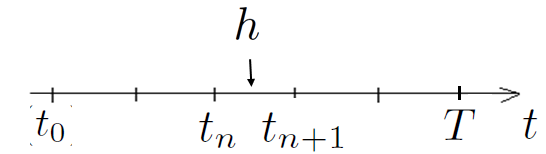
\includegraphics[width=.3\textwidth]{img/approssimazione-cauchy.png}
	\end{figure}
	
	\item Si scrive il problema di Cauchy per il generico nodo $t_{n}$ valido per ogni $n = 1, \dots, N = \frac{T}{h}$:
	\begin{equation*}
		y'\left(t_{n}\right) = f\left(t_{n}, y\left(t_{n}\right)\right)
	\end{equation*}
	
	\item Si sostituisce per ogni $n$ a $y'\left(t_{n}\right)$ una delle approssimazioni presentate: in avanti (eq. \ref{eq: approssimazione in avanti della derivata prima}), all'indietro (eq. \ref{eq: approssimazione all'indietro della derivata prima}) o centrata (eq. \ref{eq: approssimazione centrata della derivata prima}).
	
	\item Si denota, per ogni $n$, con $u_{n}$ la soluzione del nuovo problema approssimato ottenuto, la quale è una candidata per essere una buona approssimazione di $y\left(t_{n}\right)$.
\end{enumerate}
La \textbf{soluzione approssimata} è composta in generale come:
\begin{equation*}
	\left\{u_{0} = y_{0}, u_{1}, u_{2}, \dots, u_{n}\right\}
\end{equation*}